\section{Monopole Antenna}
The first monopole prototype can be seen in Figure \ref{fig:ant1_proto1_3d}. As seen on the figure both monopole antennas were very fragile. The feed pads were too small and fragile, which caused them to brake off, also as seen on the figure.

To solve the feed pad problem, a new prototype was made with $\SI{10}{mm}\times \SI{2.5}{mm}$ feed pads. The pad size was chosen to match the final tuning PCB for the project, which can be seen in Figure \ref{fig:samanthas_board}. Furthermore a FR4 support was added under the antenna feeds to make it more robust. The new prototype can be seen in Figure \ref{fig:ant1_proto2_3d}.

\begin{figure}[htbp]
  \begin{subfigure}[b]{0.49\linewidth}
        \centering
        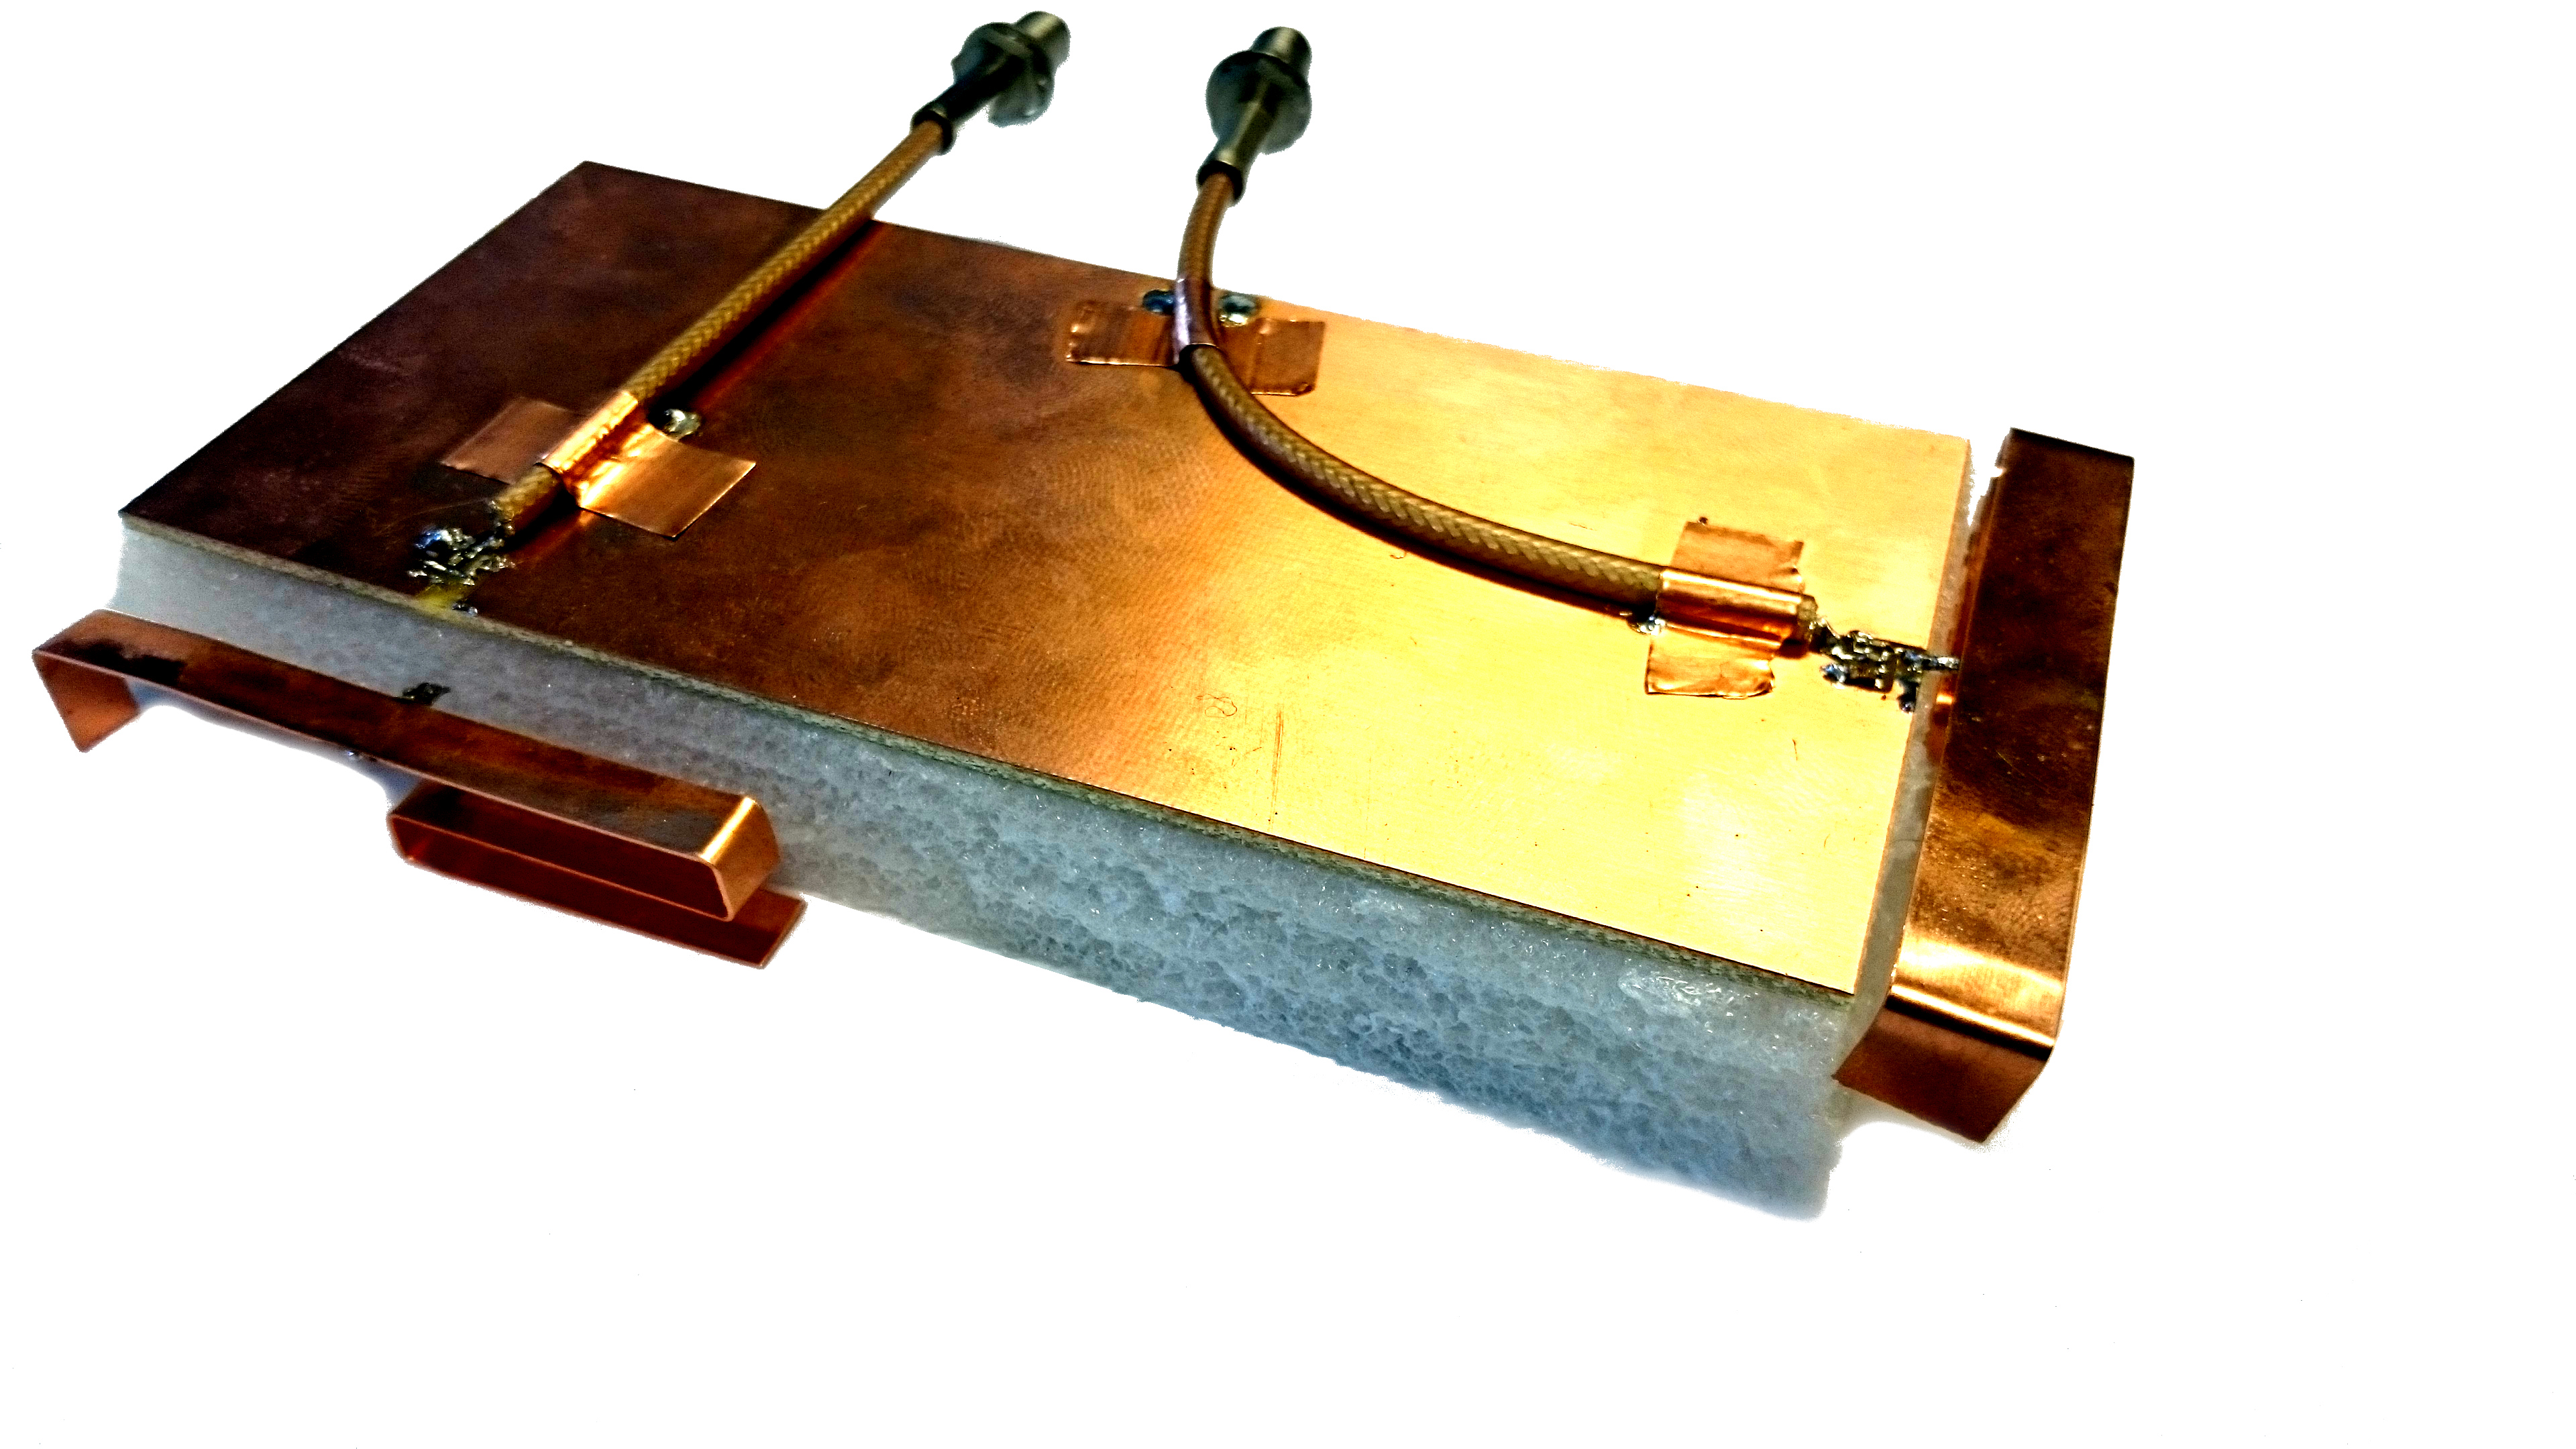
\includegraphics[scale=0.2]{img/tech_sol/monopole/prototype_v1/monopole_v1}
        \caption{Monopole prototype version 1}
        \label{fig:ant1_proto1_3d}
    \end{subfigure}
    \hfill
    \begin{subfigure}[b]{0.49\linewidth}
        \centering
        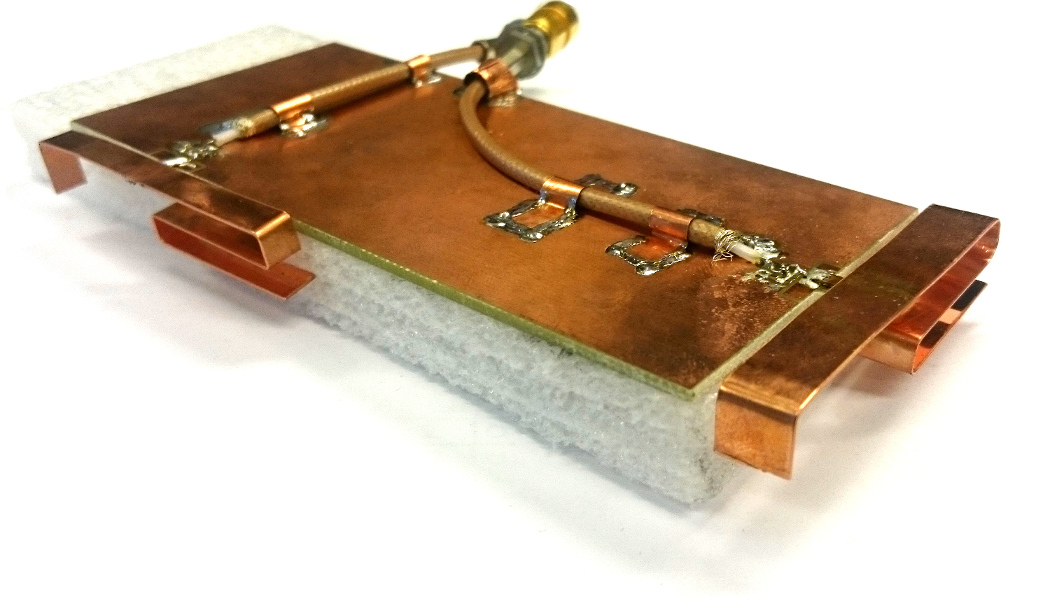
\includegraphics[scale=0.27]{img/tech_sol/monopole/prototype_v2/monopole_v2}
        \caption{Monopole prototype version 2}
        \label{fig:ant1_proto2_3d}
    \end{subfigure}
    \caption{Monopole prototype comparison of version 1 and 2}
    \label{fig:ant_1_proto_3d}
\end{figure}

\FloatBarrier
\subsection{Simulation}
The second prototype had some small changes of the feed pad and FR4 support, as described above. As a result the matching deviated some in comparison with version 1 matching simulations, which can be seen in Figure \ref{fig:sparam_mono_free_space}. To compensate for the design changes, the component values was changes accordingly. The new component values can be seen in Table \ref{fig:mono_proto_sim_matching}.

\begin{figure}[htbp]
        \centering
        \begin{tabular}{m{3in}m{3in}}
            \centering
            \includegraphics{img/tech_sol/schematic_tuning_1}&
            \centering
            \footnotesize
            \begin{tabular}{|l|l|l|l|}
                \hline
                & $C_1$ & $L_1$ & $C_2$ \\
                \hline
                Top antenna & \SI{6.5}{pF} & \SI{7}{nH} & \SI{0.3}{pF} \\
                Side antenna & \SI{2.7}{pF} & \SI{4.9}{nH} & \SI{0.3}{pF} \\
                \hline
            \end{tabular}
        \end{tabular}
    \caption{Matching circuit for the simulation prototype monopole antenna. These are the component values where the bandwidth is found to be the largest.}
    \label{fig:mono_proto_sim_matching}
\end{figure}

The S-parameter sweep of the new design can be seen on Figure \ref{fig:sparam_mono_proto_sim}. In comparison with the S11 and S22 results, the spectrum coverage for the top antenna has been slightly improved. The improvement is significant in the high band, where the top antenna now covers from \SI{1500}{MHz} to \SI{3000}{MHz}, only with a small decrease of \SI{-1}{dB} around \SI{2500}{MHz.}. The side antenna also shows spectrum improvement in the high band, but lacks some coverage of approx \SI{-3}{dB} from \SI{1710}{MHz} to \SI{1800}{MHz}. Generally the low band coverage for both antennas compared with version 1, have decreased but still covers the band.

\begin{figure}[htbp]
   \begin{subfigure}[b]{0.49\linewidth}
        \centering
        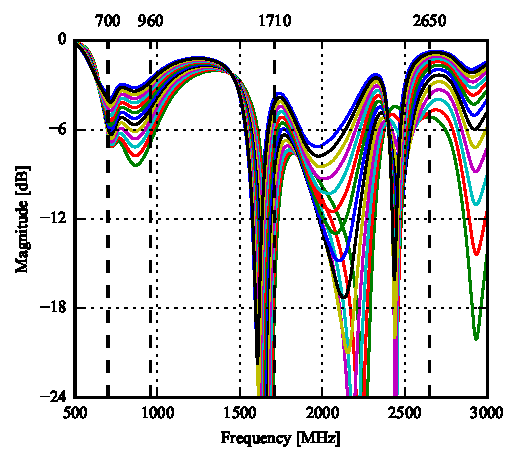
\includegraphics{img/tech_sol/monopole/prototype_v2/sim_s11}
        \caption{$S_{11}$, sweeping $C_1$ and fixing $C_2$.}
        \label{fig:ant1_proto_sim_s11}
    \end{subfigure}
    \hfill
    \begin{subfigure}[b]{0.49\linewidth}
        \centering
        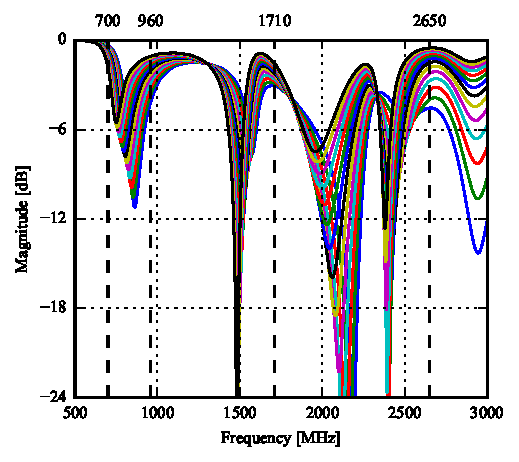
\includegraphics{img/tech_sol/monopole/prototype_v2/sim_s22}
        \caption{$S_{22}$, sweeping $C_2$ and fixing $C_1$.}
        \label{fig:ant1_proto_sim_s22}
    \end{subfigure}
~
    \begin{subfigure}[b]{0.49\linewidth}
        \centering
        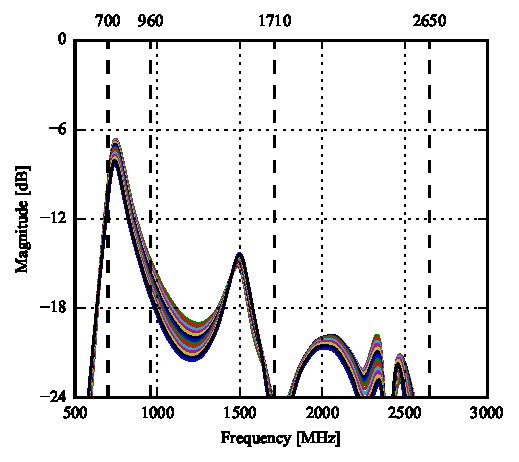
\includegraphics{img/tech_sol/monopole/prototype_v2/sim_s12_s11}
        \caption{$S_{21}$, sweeping $C_1$ and fixing $C_2$.}
        \label{fig:ant1_proto_sim_s11_s12}
    \end{subfigure}
    \hfill
    \begin{subfigure}[b]{0.49\linewidth}
        \centering
        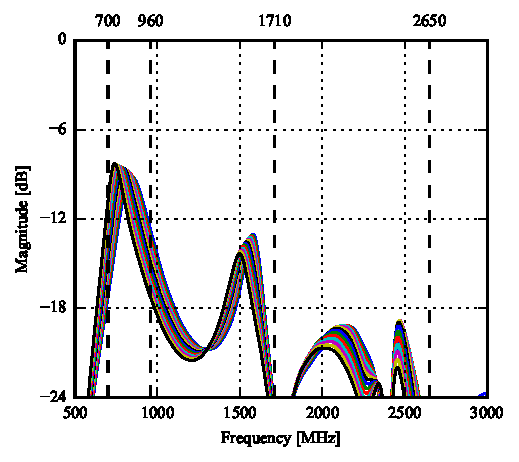
\includegraphics{img/tech_sol/monopole/prototype_v2/sim_s12_s22}
        \caption{$S_{21}$, sweeping $C_2$ and fixing $C_1$.}
        \label{fig:ant1_proto_sim_s22_s12}
    \end{subfigure}
    \caption{S-parameter sweep in free space for tuning the shunt capacitor of each antenna, $C_1$ and $C_2$ for port 1 and 2, respectively. Port 1 is the top antenna and port 2 is the side antenna.}
    \label{fig:sparam_mono_proto_sim}
\end{figure}

\FloatBarrier
\subsection{Measurements}
A comparison between the simulated and measured S-parameters can be seen on Figure \ref{fig:mono_proto_sparam_eff}. The simulated and measured results are done with the tunable capacitor at \SI{0.3}{pF}. Furthermore some component values were changes going from the simulation environment to the prototype. The prototype component values can be seen in Table \ref{fig:mono_proto_meas_matching}. Measuring the S-parameter and Efficiency sweep it was found, that the highest bandwidth was achieved with the tunable capacitor at \SI{0.3}{pF}. The bandwidth results for the top and side antenna, can be seen in Table \ref{tab:bw_sol1_proto}. From the table it is seen, that both antennas covers the required bandwidth in the low band, but have some troubles in the high band. 

The total efficiency measured and simulated with the tunable capacitors at \SI{0.3}{pF} can be seen on Figure \ref{fig:mono_proto_sparam_eff}. Generally the simulation results, shows a higher efficiency as expected. The lowest efficiencies are measured at \SI{2400}{MHz} and from \SI{700}{MHz} to \SI{750}{MHz} with the lowest efficiency at \SI{15}{\percent}. Overall the top antenna shows the best results, but still have some problems in the low band, where the efficiency drops to \SI{25}{\percent}.

\begin{figure}[htbp]
        \centering
        \begin{tabular}{m{3in}m{3in}}
            \centering
            \includegraphics{img/tech_sol/schematic_tuning_1}&
            \centering
            \footnotesize
            \begin{tabular}{|l|l|l|l|}
                \hline
                & $C_1$ & $L_1$ & $C_2$ \\
                \hline
                Top antenna & \SI{2.2}{pF} & \SI{3.3}{nH} & \SI{0.3}{pF} \\
                Side antenna & \SI{3.3}{pF} & \SI{1.2}{nH} & \SI{0.3}{pF} \\
                \hline
            \end{tabular}
        \end{tabular}
    \caption{Matching circuit for the measured prototype monopole antenna. These are the component values where the bandwidth is found to be the largest.}
    \label{fig:mono_proto_meas_matching}
\end{figure}

\begin{figure}[htbp]
    \centering
    \begin{subfigure}{0.49\linewidth}
        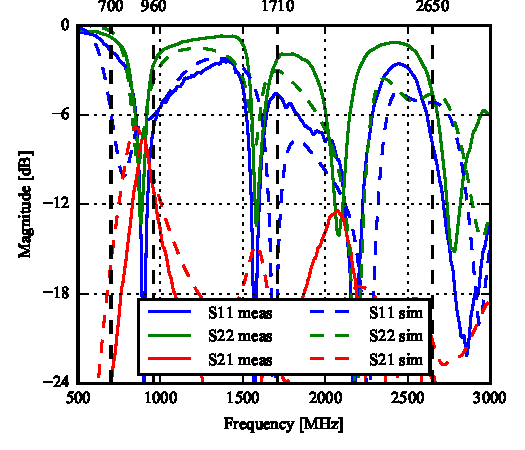
\includegraphics{img/tech_sol/monopole/prototype_v2/meas_sim_sparams.pdf}
        \caption{S-parameters.}
    \end{subfigure}
    \hfill
    \begin{subfigure}{0.49\linewidth}
        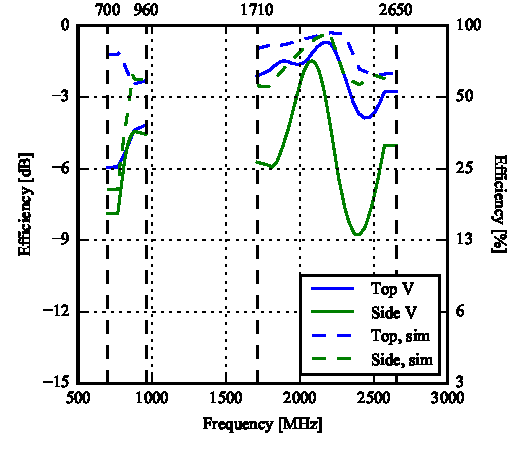
\includegraphics{img/tech_sol/monopole/prototype_v2/meas_sim_efficiency.pdf}
        \caption{Total efficiency.}
    \end{subfigure}
    \caption{S-parameters and total efficiency of the monopole antenna prototype with the component values from Figure~\ref{fig:mono_proto_sim_matching}.}
    \label{fig:mono_proto_sparam_eff}
\end{figure}

    \begin{table}
      \centering
      \begin{tabular}{|l|l|r|r|r|}
        \hline
        Antenna & Band & Start [MHz] & Stop [MHz] & Bandwidth [MHz] \\
        \hline
        Top     & Low  & 830        & 1000       & 170 \\
        Side    & Low  & 830         & 930        & 100 \\
        \hline
        Top     & High & 1800        & 2300       & 500 \\
        Side    & High & 2650        & 3000       & 300 \\
        \hline
      \end{tabular}
      \caption{Maximum bandwidth obtained in the low and high band for the top and the side antenna, respectively.}
      \label{tab:bw_sol1_proto}
    \end{table}

%S-parameter sweep
The S-parameter sweep for both antennas can be seen in Figure \ref{fig:sparam_mono_proto_sim}. The sweep is done accordingly to \ref{cha:prototypes}. From the results it can be seen that sweeping the tunable capacitors, the antennas are capable of covering most of the required bandwidth at \SI{-6}{dB}. However both the top and side antenna experiences some problems in the high band. The top antenna is able to cover the required bandwidth except at \SI{2300}{MHz}, where the magnitude drops to \SI{-3}{dB}. The side antenna experiences a magnitude drop in the high band around \SI{2200}{MHz} and \SI{2450}{MHz}. The side antenna also experiences some bandwidth problems in the low band, which makes it unable to sufficiently cover the band limit at \SI{960}{MHz}. Some of the coverage problems, especially in the high band, is likely to disappear if the sweeps were done with the same component values as used in the simulation.   

The isolation loss results shows the highest isolation loss in the low band, at approx. \SI{800}{MHz} to \SI{900}{MHz} for both the top and side antenna. This results is as expected when compared with the simulation results.
    \begin{figure}[htbp]
   \begin{subfigure}[b]{0.49\linewidth}
        \centering
        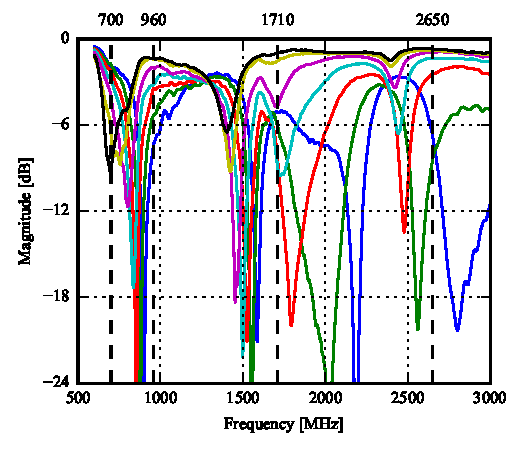
\includegraphics{img/tech_sol/monopole/prototype_v2/meas_s11_csh1}
        \caption{$S_{11}$, sweeping $C_1$ and fixing $C_2$.}
        \label{fig:ant1_proto_meas_s11}
    \end{subfigure}
    \hfill
    \begin{subfigure}[b]{0.49\linewidth}
        \centering
        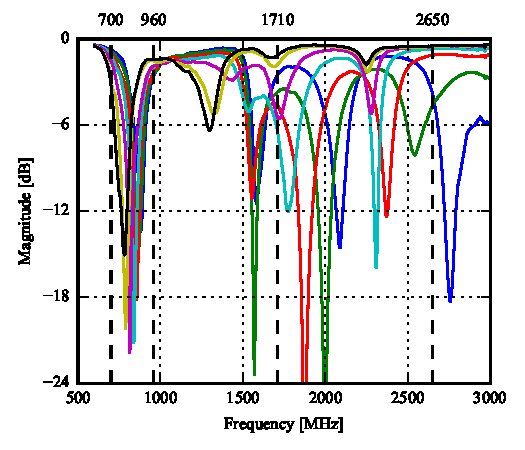
\includegraphics{img/tech_sol/monopole/prototype_v2/meas_s22_csh2}
        \caption{$S_{22}$, sweeping $C_2$ and fixing $C_1$.}
        \label{fig:ant1_proto_meas_s22}
    \end{subfigure}
~
    \begin{subfigure}[b]{0.49\linewidth}
        \centering
        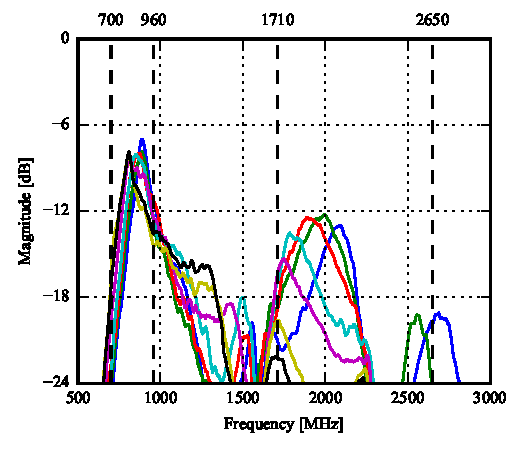
\includegraphics{img/tech_sol/monopole/prototype_v2/meas_s12_csh1}
        \caption{$S_{21}$, sweeping $C_1$ and fixing $C_2$.}
        \label{fig:ant1_proto_meas_s12}
    \end{subfigure}
    \hfill
    \begin{subfigure}[b]{0.49\linewidth}
        \centering
        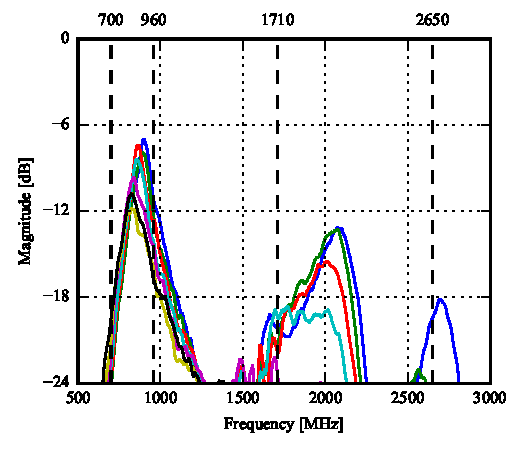
\includegraphics{img/tech_sol/monopole/prototype_v2/meas_s21_csh1}
        \caption{$S_{21}$, sweeping $C_2$ and fixing $C_1$.}
        \label{fig:ant1_proto_meas_s21}
    \end{subfigure}
    \caption{S-parameter sweep in free space for tuning the shunt capacitor of each antenna, $C_1$ and $C_2$ for port 1 and 2, respectively. Port 1 is the top antenna and port 2 is the side antenna.}
    \label{fig:sparam_mono_proto_sim}
\end{figure}
% Efficiency sweep and correlation

The efficiency sweep can be seen on Figure \ref{fig:eff_mono_proto_meas}. The sweep is done accordingly to \ref{cha:prototypes} as with the s-parameter sweeps. Looking at the results it is clearly that none of the antennas fulfill the efficiency requirements. The top antenna is able to exceed \SI{50}{\percent} efficiency in the high band, in some of the sweep modes. The side antenna shows slightly lower efficiency results compared to the top antenna. Overall both antennas decreases to \SI{3}{\percent} and below for the side antenna. This is in the worst case, but could cause some problems as every sweep mode is needed in covering the entire bandwidth. 

The correlation between the top and side antenna, can be seen on Figure \ref{fig:ant1_proto_corr}. The correlation is simulated and measured with the sweeping capacitor at the initial value of \SI{0.3}{pF}, for both the top and side antenna. From the figure it is seen, that the most significant difference in the simulated and measured correlation is in the low band at approx. \SI{830}{MHz} to \SI{960}{MHz}. Within this frequency range the simulated correlation is approx. $0.25$ higher than the measured value.

\begin{figure}[htbp]
   \begin{subfigure}[b]{0.49\linewidth}
        \centering
        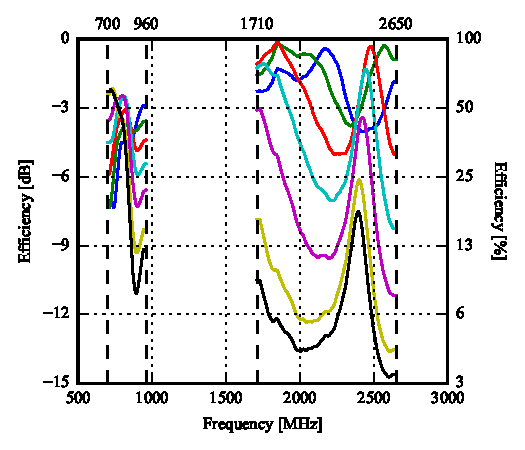
\includegraphics{img/tech_sol/monopole/prototype_v2/meas_efficiency_top}
        \caption{Efficiency for the top antenna, sweeping $C_1$ and fixing $C_2$.}
        \label{fig:ant1_proto_meas_topeff}
    \end{subfigure}
    \hfill
    \begin{subfigure}[b]{0.49\linewidth}
        \centering
        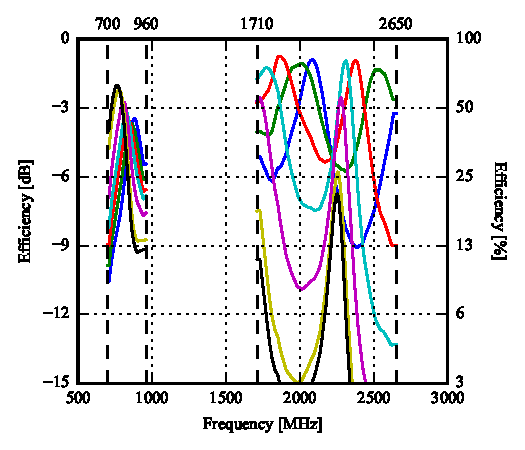
\includegraphics{img/tech_sol/monopole/prototype_v2/meas_efficiency_side}
        \caption{Efficiency for the side antenna, sweeping $C_2$ and fixing $C_1$.}
        \label{fig:ant1_proto_meas_sideeff}
    \end{subfigure}
    \caption{Efficiency sweeps in free space for tuning the shunt capacitor of each antenna, $C_1$ and $C_2$ for port 1 and 2, respectively. Port 1 is the top antenna and port 2 is the side antenna.}
    \label{fig:eff_mono_proto_meas}
\end{figure}

\begin{figure}[htbp]
    \centering
    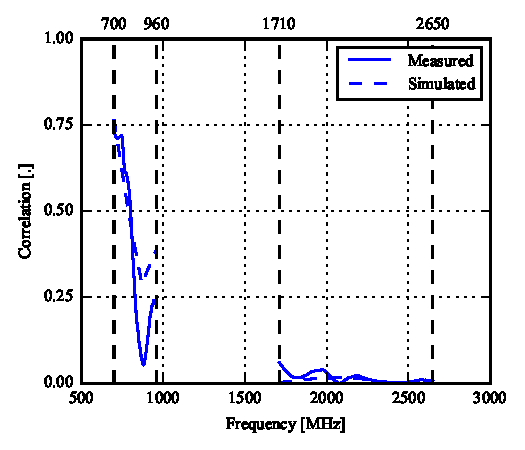
\includegraphics{img/tech_sol/monopole/prototype_v2/meas_sim_corr}
    \caption{Correlation between the top and side antenna, with $C_2=\SI{0.3}{pF}$ for both antennas.}
    \label{fig:ant1_proto_corr}
\end{figure}
